\documentclass{ctexart}
\usepackage{amsmath}
\usepackage{tikz}
\usetikzlibrary{calc,intersections}
\definecolor{star}{RGB}{13,171,160}
\begin{document}

\begin{tikzpicture}
    % 五星
    \coordinate (O) at (0,0);
    \coordinate (A) at (0,2);
    \coordinate (B) at ($(O)!1!72:(A)$);
    \coordinate (C) at ($(O)!1!72:(B)$);
    \coordinate (D) at ($(O)!1!72:(C)$);
    \coordinate (E) at ($(O)!1!72:(D)$);
    \path[name path=AC](A) -- (C);
    \path[name path=AD](A) -- (D);
    \path[name path=BD](B) -- (D);
    \path[name path=BE](B) -- (E);
    \path[name path=CE](C) -- (E);

    \path[name intersections={of=AC and BE,by=F}];
    \path[name intersections={of=AC and BD,by=G}];
    \path[name intersections={of=BD and CE,by=H}];
    \path[name intersections={of=AD and CE,by=I}];
    \path[name intersections={of=AD and BE,by=J}];
    \fill[color=star] (A) -- (F) -- (B) -- (G) -- (C) -- (H) -- (D) -- (I) -- (E) -- (J) -- cycle;
\end{tikzpicture}\vspace{2cm}

\begin{tikzpicture}[scale=1,transform shape,line width=0.6]
    % 家用机械电能表
    % 外框
    \filldraw[fill=black!20,rounded corners=2pt] (-1.5cm-8pt,-1.8cm-8pt) rectangle (1.5cm+8pt,1.8cm+8pt);
    \filldraw[fill=white,rounded corners=2pt] (-1.5,-1.8) rectangle (1.5,1.8);
    \node at (0,1.38){\small kW\:$\boldsymbol{\cdot}$\:h};
    % 度数
    \foreach \delta in {0,1,2,3,4}{
        \draw (-1.25+0.5*\delta,0.3) rectangle (-0.75+0.5*\delta,0.9);
    }
    \draw (0.8,0.35) rectangle (1.2,.85);
    \node at (-1,0.6){0};
    \node at (-0.5,0.6){6};
    \node at (0,0.6){3};
    \node at (0.5,0.6){3};
    \node at (1,0.6){5};

    % 机械轮
    % 主线条
    \draw[-{Stealth[scale=0.88]},line width=0.6pt] (-1,-0.3) -- (1,-0.3);
    % 尾部
    \filldraw (-1,-0.35) arc [start angle=-90,end angle=90,x radius=0.2,y radius=0.05];
    \filldraw[fill=white,color=white] (-1.06,-0.368) arc [start angle=-90,end angle=90,x radius=0.136,y radius=0.068];
    % 转动轮外框
    \filldraw[fill=white,rounded corners=2pt] (-0.6,-0.4) rectangle (0.6,-0.2);
    % 转动轮
    \draw[line width=1.2pt,rounded corners=.6pt] (-0.5,-0.3) -- (0.5,-0.3);

    % 规格
    \node at (0,-1){\scriptsize 220V\; 10A(20A)\; 50Hz};
    \node at (0,-1.4){\scriptsize 3\:000\:revs/(kW\:$\boldsymbol{\cdot}$\:h)};
\end{tikzpicture}\vspace{2cm}

\begin{tikzpicture}[scale=1,transform shape]
    % 家用电子电能表
    % 外框
    \filldraw[fill=black!20,rounded corners=2pt] (-1.5cm-8pt,-1.8cm-8pt) rectangle (1.5cm+8pt,1.8cm+8pt);
    \filldraw[fill=white,rounded corners=2pt] (-1.5,-1.8) rectangle (1.5,1.8);
    \node at (0,1.38){\small kW\:$\boldsymbol{\cdot}$\:h};
    % 度数
    \foreach \delta in {0,1,2,3,4}{
        \draw (-1.25+0.5*\delta,0.4) rectangle (-0.75+0.5*\delta,1);
    }
    \draw (0.8,0.45) rectangle (1.2,.95);
    \node at (-1,0.7){2};
    \node at (-0.5,0.7){8};
    \node at (0,0.7){1};
    \node at (0.5,0.7){8};
    \node at (1,0.7){6};
    % 灯光
    \filldraw[fill=red!100,draw=white] (-0.3,0.1) circle [radius=2pt];
    \node at (0.2,0.1){\scriptsize 脉冲};
    % 文字
    \node at (0,-0.3){\small 电子式单向电能表};
    % 规格
    \node at (0,-1){\scriptsize 220V\; 10A(20A)\; 50Hz};
    \node at (0,-1.4){\scriptsize 1\:200\:imp/(kW\:$\boldsymbol{\cdot}$\:h)};
\end{tikzpicture}\vspace{2cm}

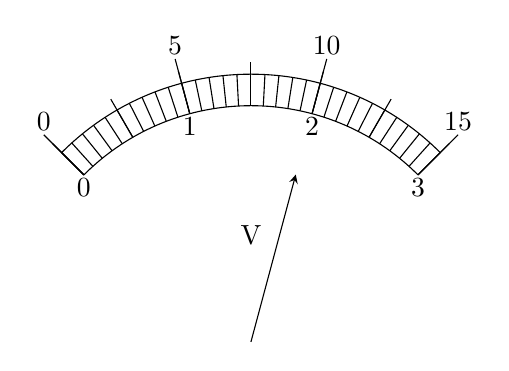
\begin{tikzpicture}
    % 电压表
    \draw (45:3) arc [start angle=45,end angle=135,radius=3];
    \draw (45:3.4) arc [start angle=45,end angle=135,radius=3.4];
    \foreach \smalls in {45,48,...,135}{
        \draw (\smalls:3) -- (\smalls:3.4);
    }
    \foreach \bigs in {45,60,...,135}{
        \draw (\bigs:3) -- (\bigs:3.56);
    }
    \foreach \bbigs/\snum/\bnum in {45/3/15,75/2/10,105/1/5,135/0/0}{
        \draw (\bbigs:3) -- (\bbigs:3.72);
        \node[below=-2pt] at (\bbigs:3){\snum};
        \node[above=-2pt] at (\bbigs:3.72){\bnum};
    }
    \draw[-stealth] (0,0) -- (75:2.2);
    \node at (0,1.36){V};
\end{tikzpicture}\vspace{2cm}

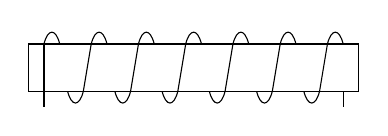
\begin{tikzpicture}
    % 螺线管1(左现右隐)
    \draw (-2,-0.3) rectangle (2.2,0.3);
    % 螺线
    \draw (-1.8,-0.5) -- (-1.8,0.3);
    \foreach \x in {-1.8,-1.2,-0.6,0,0.6,1.2}{
        \draw (\x,0.3) .. controls (\x+0.05,0.5) and (\x+0.15,0.5) .. (\x+0.2,0.3);
        \draw (\x+0.3,-0.3) ..controls (\x+0.35,-0.5) and (\x+0.45,-0.5) .. (\x+0.5,-0.3);
        \draw (\x+0.5,-0.3) -- (\x+0.6,0.3);
    }
    \draw (1.8,0.3) .. controls (1.85,0.5) and (1.95,0.5) .. (2,0.3);
    \draw (2,-0.3) -- (2,-0.5);
\end{tikzpicture}\vspace{2cm}

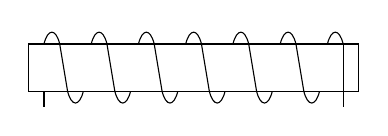
\begin{tikzpicture}
    % 螺线管2(左隐右现)
    \draw (-2,-0.3) rectangle (2.2,0.3);
    % 螺线
    \draw (-1.8,-0.5) -- (-1.8,-0.3);
    \foreach \x in {-1.8,-1.2,-0.6,0,0.6,1.2}{
        \draw (\x,0.3) .. controls (\x+0.05,0.5) and (\x+0.15,0.5) .. (\x+0.2,0.3);
        \draw (\x+0.2,0.3) -- (\x+0.3,-0.3);
        \draw (\x+0.3,-0.3) ..controls (\x+0.35,-0.5) and (\x+0.45,-0.5) .. (\x+0.5,-0.3);
    }
    \draw (1.8,0.3) .. controls (1.85,0.5) and (1.95,0.5) .. (2,0.3);
    \draw (2,0.3) -- (2,-0.5);
\end{tikzpicture}\vspace{2cm}

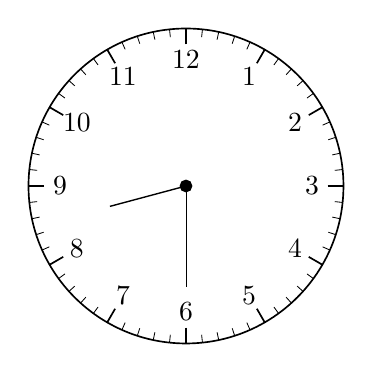
\begin{tikzpicture}[line width=0.6pt]
    % 圆时钟
    \draw (0,0) circle [radius=2cm];
    \foreach \r in {0,6,...,354}{
        \draw[line width=0.3pt] (\r:1.9) -- (\r:2);
    }
    \foreach \r/\n in {0/3,30/2,60/1,90/12,120/11,150/10,180/9,210/8,240/7,270/6,300/5,330/4}{
        \draw (\r:1.8) -- (\r:2);
        \node at (\r:1.6){\n};
    }
    \filldraw (0,0) circle [radius=2pt];
    \draw[line width=0.25pt] (0,0) -- (270:1.28);
    \draw[line width=0.5pt] (0,0) -- (195:1);
\end{tikzpicture}
\end{document}

